\chapter{Preliminares}

\section{Medidas y unidades}
Las cantidades básicas en mecánica son longitud [L], masa [M] y tiempo [T], en donde se ha usado una letra entre corchete para denotar el símbolo dimensional de la cantidad física. En el Sistema Internacional (SI) de unidades están cantidades se miden en metros ($\meter$), kilogramos ($\kilo\gram$) y segundos ($\second$).
\begin{itemize}
\item Un segundo es la duración de $9\ 192\ 631\ 770$ oscilaciones de la radiación emitida en la transición entre los dos niveles hiperfinos del estado fundamental del isótopo 133 del átomo de cesio (${}^{133}$Cs), a una temperatura de 0 K~\cite{wikipedia}
\item Un metro es la distancia que recorre la luz en el vacío durante un intervalo de $1/299\ 792\ 458$ de segundo~\cite{wikipedia}
\item Un kilogramo es la masa que tiene el prototipo internacional, compuesto de una aleación de platino e iridio, que se guarda en la Oficina Internacional de Pesas y Medidas (BIPM) en Sèvres, cerca de París (Francia)~\cite{wikipedia}.
Es la única unidad del SI que todavía se define por un objeto patrón y no por una característica física fundamental.
\end{itemize}





\section{Vectores}
\label{sec:vectores}

Las cantidades completamente especificadas por su magnitud se llaman escalares. Ejemplos de escalares son la masa, temperatura, rapidez, etc.

Hemos visto que tanto la posición, como la velocidad y la aceleración, no sólo tienen asociadas una magnitud, sino también una dirección. Un ejemplo de vector corresponde al asociado a la aceleración gravitacional el cual tiene una magnitud de $9.8\ \text{m}/\text{s}^2$.

\subsection{Aproximación geométrica a vectores}

Ejemplos de vectores: magnitud y direcci\'on
\begin{itemize}
\item Desplazamiento [$\text{L}$]
\item Velocidad [$\text{L/T}$] 
\item Aceleración [$\text{L/T}^2$]
\item Fuerza [$\text{M L/T}^2$]
\item Moméntum [$\text{M L/T}$]
\item Moméntum angular [$\text{M\,L}^2/\text{T}$]
\item Torque [$\text{M\,L}^2/\text{T}^2$]
\end{itemize}

Una característica muy importante de los vectores es que sus propiedades de magnitud y dirección son independientes del sistema de coordenadas elegido. En términos vectoriales, dos desplazamientos hacia el norte de 3 metros son completamente equivalentes. 



Ejemplos de escalares: magnitud pero no dirección
\begin{itemize}
\item Longitud [$\text{L}$]
\item Tiempo [$\text{T}$]
\item Masa [$\text{M}$]
\item Área [$\text{L}^2$]
\item Volumen [$\text{L}^3$]
\item Densidad [$\text{M/L}^3$]
\item Energía [$\text{M\,L}^2/\text{T}^2$]
\item Temperatura [$\mathcal{T}$]
\end{itemize}

\begin{align*}
  \mathbf{A}=&\mathbf{B} &\qquad \text{si}\qquad |\mathbf{A}|&=|\mathbf{B}|\nonumber\\
  &&|\mathbf{A}|&\parallel|\mathbf{B}|\,.
\end{align*}
Adem\'as
\begin{align}
  A\equiv|\mathbf{A}|\,.
\end{align}

\textbf{Suma de vectores}
ver \href{https://docs.google.com/viewer?a=v&pid=sites&srcid=ZmlzaWNhLnVkZWEuZWR1LmNvfG1lY2FuaWNhfGd4OjdmNWMyZTc5NDIxNTAxNjg}{vectores.pdf}
\begin{inprogress}
  inkscape: ley conmutativa
\end{inprogress}
Suma s\'olo tiene sentido para el mismo para el mismo tipo de vectores


\subsection{Aproximaci\'on algrebr\'aica  a vectores}

\begin{frame}[fragile,allowframebreaks]
Un vector en el plano $x-y$, con vectores unitarios $\hat{\mathbf{i}}$ en la direcci\'on $x$, $\hat{\mathbf{j}}$ en la direcci\'on $j$, y  formando un \'angulo $\theta$ con el eje $x$ se puede visualizar como la suma de dos vectores:
\begin{align}
  \mathbf{A}=&\mathbf{A}_x+\mathbf{A}_y\nonumber\\
            =&A_x\hat{\mathbf{i}}+A_y\hat{\mathbf{j}}\nonumber\\
            =&(A_x,A_y)\nonumber\\
            =&(A_1,A_2).
\end{align}
En t\'erminos de componentes
\begin{align}
  \mathbf{A}_i=A_i\,.
\end{align}

El vector $\mathbf{A}$ está represantado en la figura \ref{fig:avec}
\begin{figure}
  \centering
  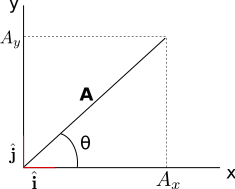
\includegraphics[scale=1]{avec}
  \caption{Vector $\mathbf{A}$}
\label{fig:avec}
\end{figure}


La magnitud al cuadrado del vector se obtiene del teorema de Pitagoras
\begin{align}
  \label{eq:pitagoras}
  \mathbf{A}\cdot\mathbf{A}\equiv|\mathbf{A}|^2=A^2=&A_x^2+A_y^2\nonumber\\
  =&\sum_{i=1}A_i^2\,.
\end{align}
Definiendo el delta de Kronecker como
\begin{align}
  \delta_{ij}=
  \begin{cases}
    1&\text{si $i=j$}\\
    0&\text{si $i\neq j$}\\
  \end{cases}
\end{align}
podemos escribir la magnitud al cuadrado del vector $\mathbf{A}$ de una forma que se puede generalizar facilmente a $n$-dimensiones. Para $n=3$ por ejemplo:
\begin{align}
   A^2=\mathbf{A}\cdot\mathbf{A} =&\sum_{i,j=1}^3A_i A_j\delta_{ij}\nonumber\\
   =&\sum_{i=1}^3\left(A_iA_1\delta_{i1}+A_iA_2\delta_{i2}+A_iA_1\delta_{i3}\right)\nonumber\\
   % falta un paso
   =&A_1A_1\delta_{11}+A_2A_2\delta_{22}+A_3A_3\delta_{33}\nonumber\\
   =&A_1^2+A_2^2+A_3^2\nonumber\\
   =&\sum_{i=1}^3A_i^2\,.
\end{align}
Teniendo en cuenta el \'angulo $\theta$ definido en la figura \ref{fig:avec} en la ec.\eqref{eq:pitagoras}, tenemos que
\begin{align}
  A_x=&|\mathbf{A}|\cos\theta=A\cos\theta\nonumber\\
  A_y=&|\mathbf{A}|\sin\theta=A\sin\theta\,,
\end{align}
De modo que
\begin{align}
  \tan\theta=\frac{A_y}{A_x}\,,
\end{align}
y
\begin{align}
  \theta=\tan^{-1}\frac{A_y}{A_x}
\end{align}


\subsection{Vectores y escalares}


Una cantidad que es representada por un sólo número es llamada un \emph{escalar} \cite{MI}. Una cantidad escalar no tiene dirección, Ejemplos incluyen la masa de un objeto, tal como uno de 5~Kg. o una tempetatura tal como $-20^\circ\ $C. Vectores y escalares son entidades muy diferentes; un vector nunca puede ser igual a un escalar, y un escalar no se pude sumar a un vector. Los escalares pueden ser positivos o negativos:
\begin{align*}
  m=&50\ \text{Kg}\\
  T=&-20^\circ\ \text{C} 
\end{align*}

Aunque una componente de un vector tal como $A_x$ no es un vector, tampoco es un escalar, a pesar de ser sólo un número. Una propiedad muy importante de un escalar es que este no cambia si cambiamos el sistema de referencia, mientras que la componente de un vector si puede cambiar, por ejemplo si orientamos los ejes de coordenadas $x, y, z$ de una forma diferente.


\subsection{Operaciones vectoriales}

Para sumar dos vectores algebra\'\i camente, se desplazan los origenes de los dos vectores a un origen de coordenadas que coincida con el plano formado por los dos vectores, como se muestra en la figura~\ref{fig:apbvec}. Entonces es facil ver que
\begin{align}
  \mathbf{C}=\mathbf{A}+\mathbf{B}=&(A_x+B_x)\hat{\mathbf{i}}+(A_y+B_y)\hat{\mathbf{j}}\nonumber\\
  =&(A_x+B_x,A_y+B_y)\nonumber\\
  =&(A_1+B_1,A_1+B_1).
\end{align}

\begin{figure}
  \centering
  \includegraphics[scale=1]{apbvec}
  \caption{Suma algebráica de vectores}
\label{fig:apbvec}
\end{figure}
En t\'erminos de componentes:
\begin{align}
  \left(\mathbf{A}+\mathbf{B}\right)_i=A_i+B_i\,.
\end{align}
\end{frame}

%Ejemplo sonbre descomposición del peso en un plano inclinado

\begin{figure}
  \centering
  \includegraphics{planopeso1}
  \caption{Peso}
  \label{fig:planopeso1}
\end{figure}

\begin{figure}
  \centering
  \includegraphics{planopeso2} \includegraphics{planopeso3} 
  \caption{Peso}
  \label{fig:planopeso2}
\end{figure}

\begin{frame}[fragile,allowframebreaks]
Procedemos ahora a definir el \emph{producto escalar entre dos vectores} cuyo resultado es un escalar como:
\begin{align}
  \mathbf{A}\cdot\mathbf{B}\equiv&A_xB_x+A_yB_y\nonumber\\
  =&\sum_{i,j=1}^2A_iB_j\delta_{ij}\nonumber\\
  =&\sum_{i}^2A_iB_i\,,
\end{align}

El producto escalar puede escribirse en términos de la magnitud de los
vectores y el ángulo entre ellos. Para ello definimos $\beta$ como el
\'angulo entre los vectores $\mathbf{A}$ y $\mathbf{B}$. Escojemos el
sistema de coordenadas en el plano formado por los dos vectores tales
que $\alpha+\beta$ sea el \'angulo de $\mathbf{A}$ con $x$ y $\alpha$
el \'angulo de $\mathbf{B}$, como se mueste en la figura~\ref{fig:adotbvec}. 

\begin{figure}
  \centering
  \includegraphics[scale=1]{adotbvec}
  \caption{Producto escalar entre dos vectores}
  \label{fig:adotbvec}
\end{figure}

Entonces, de la definici\'on tenemos:
\begin{align}
    \mathbf{A}\cdot\mathbf{B}=&A_xB_x+A_yB_y\nonumber\\
    =&A\cos(\alpha+\beta)B\cos\alpha+A\sin(\alpha+\beta)B\sin\alpha\nonumber\\
    =&AB[(\cos\alpha\cos\beta-\sin\alpha\sin\beta)\cos\alpha+(\sin\alpha\cos\beta+\cos\alpha\sin\beta)\sin\alpha]\nonumber\\
    =&AB(\cos^2\alpha+\sin^2\alpha)\cos\beta\nonumber\\
    =&AB\cos\beta\nonumber\\
    =&|\mathbf{A}||\mathbf{B}|\cos\beta\,,
\end{align}
De este modo, el \'angulo entre dos vectores,
$\beta$, se puede obtener como
\begin{align}
  \cos\beta=\frac{\mathbf{A}\cdot\mathbf{B}}{|\mathbf{A}||\mathbf{B}|}\,.
\end{align}
\end{frame}

%ejemplo trabajo

\begin{frame}[fragile,allowframebreaks]
El producto vectorial $\mathbf{C}=\mathbf{A}\timesm\mathbf{B}$, se define algebra\'\i camente como:
\begin{align}
  C_k=\left(\mathbf{A}\timesm\mathbf{B}\right)_k=&\sum_{ij}\epsilon_{ijk}A_iB_j\,,
\end{align}
donde el s\'\i mbolo de Levi-Civita se define con respecto a las
permutaciones con referencia al orden 123 como
\begin{align}
  \epsilon_{ijk}\equiv& \begin{cases}
    0&\text{si hay \'\i ndices iguales}\\
    1&\text{permutaci\'on par}\\
    -1&\text{permutaci\'on impar}\\
  \end{cases}.
\end{align}
Entonces
\begin{align}
  C_x=C_1=\left(\mathbf{A}\timesm\mathbf{B}\right)_1=&
\sum_{i=1}^3\left(\cancel{\epsilon_{i11}}A_iB_1+\epsilon_{i21}A_iB_2+\epsilon_{i31}A_iB_3\right)\nonumber\\
=&\cancel{\epsilon_{121}}A_1B_2+\cancel{\epsilon_{221}}A_2B_2
+\epsilon_{321}A_3B_2+\cancel{\epsilon_{131}}A_1B_3\nonumber\\
&+\epsilon_{231}A_2B_3+\cancel{\epsilon_{331}}A_3B_3\,.
\end{align}
Teniendo en cuenta que $321\to231\to213\to123$ (3 permutaciones) y
$231\to213\to123$ (2 permutaciones), entonces
\begin{align}
  \epsilon_{321}=-1\,\qquad \epsilon_{231}=+1\,,
\end{align}
de modo que
\begin{align}
  C_x=C_1=&A_2B_3-A_3B_2\,.
\end{align}
Similarmente para $C_y$ y $C_z$, tenemos
%faltan detalles
\begin{align}
  \label{eq:crossprod}
  \mathbf{C}=&\left(A_yB_z-A_zB_y\right)\hat{\mathbf{i}}
-\left(A_xB_z-A_zB_x\right)\hat{\mathbf{j}}
+\left(A_xB_y-A_yB_x\right)\hat{\mathbf{k}}\nonumber\\
 =&\left(A_2B_3-A_3B_2,A_3B_1-A_1B_3,A_1B_2-A_2B_1\right)
\,.
\end{align}
Definimos
\begin{align}
  \label{eq:det}
  \mathbf{C}=\begin{vmatrix}
    \hat{\mathbf{i}} & \hat{\mathbf{j}} & \hat{\mathbf{k}}\\
    A_x & A_y & A_z\\
    B_x & B_y & B_z
  \end{vmatrix}\equiv\left(A_yB_z-A_zB_y\right)\hat{\mathbf{i}}
-\left(A_xB_z-A_zB_x\right)\hat{\mathbf{j}}
+\left(A_xB_y-A_yB_x\right)\hat{\mathbf{k}}\,.
\end{align}
El resultado (\ref{eq:crossprod}) se puede obtener tambi\'en con la
regla para calcular el determinante definido en la ec.~(\ref{eq:det}),
como se muestra en la figura~\ref{fig:cross}.
\begin{figure}
  \centering
  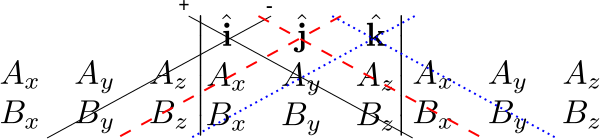
\includegraphics[scale=0.7]{cross}
  \caption{Regla para el determinante: Para cada par de l\'\i neas, el cruze de las l\'\i neas definen
    el vector unitario, que va acompa\~nado por el producto de las
    cantidades bajo la l\'\i nea de izquierda  a derecha menos el producto
    de la cantidades de derecha a izquierda. El signo menos aparece
    naturalmente para el producto asociado a $\hat{\mathbf{j}}$.  }
  \label{fig:cross}
\end{figure}

Para mostrar como el producto vectorial se reduce la definici\'on
geom\'etrica en t\'erminos de las magnitudes y el \'angulo entre los dos
vectores, considere el plano definido por los vectores $\mathbf{A}$ y
$\mathbf{B}$ que forman un \'angulo $\alpha$ entre ellos. Escojamos el eje
$x$ a lo largo del vector $\mathbf{A}$, como se muestra en la en la figura~\ref{fig:axbvec}. 

\begin{figure}
  \centering
  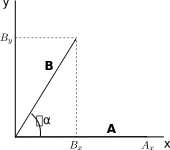
\includegraphics[scale=1]{axbvec}
  \caption{Producto escalar entre dos vectores}
  \label{fig:axbvec}
\end{figure} 

Entonces:
\begin{align}
  A_y=A_z=B_z=0\qquad A=A_x\qquad\text{y}\ B_y=B\sin\alpha\,. 
\end{align}
Por consiguiente
\begin{align}
  \mathbf{C}=\mathbf{A}\timesm\mathbf{B}=&A_xB_y\hat{\mathbf{k}}\nonumber\\
  =&A B\sin\alpha\,\hat{\mathbf{k}}\,,
\end{align}
y entonces
\begin{align}
  |\mathbf{C}|=|\mathbf{A}||\mathbf{B}|\sin\alpha\,.
\end{align}
\end{frame}

\begin{itemize}
\item[\textbf{Ejemplo:}] Sea $\mathbf{r}$ la distacia desde algún punto sobre la vertical de un círculo de radio $R$ hasta su punto más inferior: $P$, como se ilustra en la figura~\ref{fig:examplecross}. Calcule el producto escalar entre $\mathbf{r}$ y $\mathbf{f}$ cuando el punto sobre (a) la vertical está en en el centro del círculo ($C$),  (b) cuando está en el punto inferior $P$ y (c) cuando está en el punto superior. Índique claramente la dirección del vector resultante. Si $\mathbf{f}$ es una fuerza índique además el sentido del giro del círculo con un eje pasando por su centro.
  \begin{figure}
    \centering
    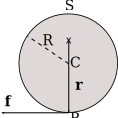
\includegraphics{examplecross}
    \caption{Ejemplo productor vectorial}
    \label{fig:examplecross}
  \end{figure}

\textbf{Solución:} Para el eje $z$ saliendo de la página (a) $\mathbf{r}\times\mathbf{f}=-R f \hat{\mathbf{k}} $, dirección horaria de giro (b) $\mathbf{r}\times\mathbf{f}=\mathbf{0}\times\mathbf{f}=\mathbf{0}$ y (c) $\mathbf{r}\times\mathbf{f}=-2R f \hat{\mathbf{k}} $, dirección horaria de giro.

\end{itemize}

\subsection{Cambio en una cantidad}

Frecuentemente queremos calcular el cambio en una cantidad. Por
ejemplo, podríamos desear conocer el cambio en la posición de un
objeto en movimiento, o el cambio en la velocidad durante un intervalo
de tiempo. La letra $\Delta$ (delta mayúscula que sugiere una ``$d$ de
diferencia'') se usa para denotar el cambio en una cantidad ya sea
escalar o vectorial.

\newpage


\qquad

\newpage

%%% Local Variables: 
%%% mode: latex
%%% TeX-master: "mecanica"
%%% End: 
